\chapter{Crystallographic Symmetry}

\section{The lattice}

Moving from interactions of quanta and matter, let us consider how atoms are arranged in matter. Atoms exist in a quantum-level universe as well, and repel each other if they are placed too close, but attract each other at longer distances. They can also create lower-energy structures by sharing electrons (chemical bonding) to form molecules or for unbonded charged objects, packing in three dimensions in a way to best alternating charge can also reduce the energy (a simple way to consider this is via the Madelung potential). 
In general, enthalpy is lowered when atoms and molecules self-arrange in dense and regular three-dimensional patterns. Opposing this is entropy, which is increased by randomness. 
In the macroscopic world that we live in, entropy and enthalpy balance at equilibrium, and all materials, even away from equilibrium, exist with both order and disorder present. 
Nonetheless, it is worthwhile considering the properties and symmetry of a perfectly organized set of atoms or molecules, which we will call an ideal crystal, even though it is an imaginary concept; no perfectly ordered materials exist. 

In an ideal crystal, atoms occur only at a set of fixed distances from each other, and the structure is built up of repeating units. 
For the purposes of this introduction, I will not consider two important forms of crystalline matter, quasicrystals and modulated structures, as these require descriptions in more than three dimensions. 
Quasicrystals are composed of atoms that organize in long-range patterns, but these patterns do not repeat in regular units. 
In 1982 Dan Shechtman\index{Schectman, D.} found clear evidence for such a material, and despite rejection from a significant and highly vocal segment of the scientific community (typified by a comment attributed to Linus Pauling\index{Pauling, L.} that “there are no quasicrystals, only quasi-scientists”) continued to speak to what he had observed in an electron microscope. 
The existence of quasicrystals\index{quasicrystal} is now fully accepted, and Shechtman was awarded a solo Nobel prize in 2011. 
Similarly, in modulated structures, incommensurate ordering is superimposed on regular three-dimensional patterns of repetition. 
While initially, the definition of what we would call crystalline matter was tied to the existence of long-range repetition units of atoms, now the definition has been expanded to any matter that shows long-range atomic organization through the appearance of a sharp diffraction pattern. 
Since my goal here is to explore the properties from long-range repetition units of atoms and show how sharp diffraction patterns arise from this, I will only consider classical three-dimensional ideal crystals and will use them to introduce two initial concepts, the lattice and the reciprocal lattice. 

Our imaginary idealized crystal is built of repeated three-dimensional identical boxes of atoms. 
At this stage, we do not need to concern ourselves with how the atoms are arranged within each box, but we will stipulate that identical means this arrangement is repeated exactly in every box. 
The crystal is built up by these boxes stacked in every direction. 
It has been known since the 1800’s that there are seven shapes of boxes that can be used to build a larger object without any gaps. 
In the simplest example this box would be a cube – having equal length sides and all angles between sides as multiples of 90 degrees. 
However, these requirements on dimensions and angles can be relaxed, giving rise to a total of seven options, as listed in the Table \ref{tab:constraints};\footnote{Note that conventionally the term rhombohedral is used for both a class of lattice symmetry, that can occur with two different types of unit cells, or a unit cell that has three equal cell lengths and cell angles; to differentiate the latter, I reserve rhombohedral for symmetry and rhombohedric for the unit cell type.} this gives rise to what is known as the \textbf{seven crystal systems}\index{crystal systems}. 
These boxes are all parallelepipeds, meaning six-sided objects where there are three pairs of parallel sides. 
Note that while one can tile space with hexagons (or in three dimensions, hexagonal prisms), we consider the hexagonal crystal systems to be constructed from parallelepipeds with two equal sides that have a 120° angle between them and where the third side is perpendicular to the other two. 
Three of these parallelepipeds can construct hexagonal prisms. 
Thus, this parallelepiped description is equivalent to one built from hexagonal prisms. 

\begin{table}
\centering
\caption{The seven crystal systems and their constraints.}
\label{tab:constraints}
\begin{tabular}{| l | p{0.25\textwidth} | p{0.4\textwidth} |}
\hline
Name & Constraints on lengths of sides & Constraints on angles between sides \\
\hline
Cubic & All three equal & All 90 degrees \\
\hline
Tetragonal & Two must be equal & All 90 degrees \\
\hline
Orthorhombic & none & All 90 degrees \\
\hline
Hexagonal & Two must be equal & 120 deg. between equal sides; 90 deg. for other two \\
\hline
Rhombohedric & All three equal & Any, but all three must be equal \\
\hline
Monoclinic & none & Any for one, 90 deg. for other two \\
\hline
Triclinic & None & None \\
\hline

\end{tabular}

\end{table}

 Armed with the concept of crystal systems, we can define an important term in crystallography, that of a \textbf{lattice}\index{lattice}. 
Let us label one arbitrary point in the box. 
The point we select might be a corner but could also be some location inside the box. 
For that selected point, we can envision that there will be a fixed arrangement of atoms around that point. 
Should we move to the same point in any other box, the arrangement of atoms will be identical since the boxes are all identical. 
If we then imagine selecting that same point in every box, we construct an infinite network of indistinguishable points. This infinite network of points is called the lattice. For a given arrangement of atoms, there are any number of ways to construct the lattice, since we can choose any point in the box as our reference point. We could also choose a more sparse network of points, such as selecting every other point in some direction and thus enlarge our box, but still we can decorate our infinite crystal from that lattice. Thus, there are an infinite number of possible lattices associated with a structure. We will see later that only some will better describe the symmetry of the structure. The term lattice is commonly misused to describe the structure or chemical makeup of the crystal, with poorly considered terms such as “lattice compound.” In truth, a lattice is just a mathematical concept, simply a collection of points. 

\section{The unit cell and fractional coordinates}

 For the box we used to construct our ideal crystal, we give the name the \textbf{unit cell.}\index{unit cell}
 We still need not consider exactly how the atoms are arranged within that box, but since every box (or equivalently unit cell) is identical, once we have described the contents of the unit cell, we can construct an exact description of the entire crystal. 
 This leads to a very convenient mechanism for describing the coordinates of atoms within the unit cell using \textbf{crystallographic axes}, which are also sometimes called the \textbf{crystal axes}. We label the three sides of the unit cell as \textbf{\textit{a}, \textit{b} \& \textit{c}}\index{\textit{a}}\index{\textit{b}}\index{\textit{c}}, and define the angles between the sides as \textbf{α}, \textbf{β}, \& \textbf{γ}\index{$\alpha$}\index{$\beta$}\index{$\gamma$}, where we define as γ the angle between the \textit{a} \& \textit{b} sides, β between \textit{a }\& \textit{c}, and α between \textit{b} \& \textit{c}. We then define \textbf{axes}, \textbf{x, y \& z} along \textit{a}, \textit{b} \& \textit{c} directions, respectively. Note that the angles between these axes are dictated by α, β \& γ, so for systems other than cubic, tetragonal and orthorhombic, angles between axes may not be 90 degrees. Such axes systems are \textit{non-orthogonal} (also called oblique) which makes performing three-dimensional algebra more difficult, but will so greatly simplify our descriptions of the crystal that this mechanism is much preferred over orthogonal coordinate systems. Table \ref{tab:conventions} outlines the common conventions used for assigning axes for the seven crystal systems.
 
\begin{table}
\centering
\caption{Conventions for labeling of axes for the seven crystal systems.\index{crystal systems} Note that for monoclinic systems, the convention below is the current conventional preference, but \textit{c} unique (where α = β = 90°) was more commonly used historically. Use of \textit{a} unique (β = γ = 90°) is seen in the literature only rarely.}
\label{tab:conventions}

\begin{tabular}{| l | p{0.2\textwidth} | p{0.3\textwidth} |}

\hline
Crystal system name & Constraints on lengths of sides & Constraints on angles between sides \\
\hline
Cubic & \textit{a}=\textit{b}=\textit{c} & α = β = γ = 90° \\
\hline
Tetragonal & \textit{a}=\textit{b} & α = β = γ = 90° \\
\hline
Orthorhombic & none & α = β = γ = 90° \\
\hline
Hexagonal & \textit{a}=\textit{b} & γ = 120°; α = β = 90° \\
\hline
Rhombohedric & \textit{a}=\textit{b}=\textit{c} & α = β = γ \\
\hline
Monoclinic & none & b unique: α = γ = 90° \\
\hline
Triclinic & none & none \\
\hline

\end{tabular}

\end{table}

 Finally, we scale each axis so that one unit of length corresponds to the length of the unit cell in that direction. This means that for most crystal systems the per unit along each axis may differ, so This means that we can label any point inside the unit cell with coordinates (x,y,z) where $0\leq \rm x<1$, $0\leq \rm y<1$ and $0\leq\rm z<1$. Locations on the faces of the unit cell will have $\rm x=0$ or $\rm y=0$ or $\rm z=0$ and the coordinates for the eight corners of the unit cell are (0,0,0), (1,0,0), (0,1,0), (0,1,0), (1,1,0), (1,0,1), (0,1,1) and (1,1,1). The center of the unit cell is (0.5, 0.5, 0.5). This system of coordinates is known as \textbf{fractional coordinates}.\index{fractional coordinates} We can also consider the location of a point inside the cell with location (x,y,z) as a vector from the origin to the atom position, $\vec{x_{xyz}}=\ x\hat{a}+\ y\hat{b}+z\hat{c}$ where $\hat{a}$, $\hat{b}$ and $\hat{c}$ are unit vectors (\textit{i.e.} with length in the same units, for example, Å) in the appropriate direction.

 Note that since the contents of every unit cell is the same, adding or subtracting any multiple of 1 to x, y and/or z results in a location that is indistinguishable from the initial point. We can write a rule that point (x,y,z) is equivalent to (x+n\textsubscript{x}, y+n\textsubscript{y}, z+n\textsubscript{z}) where n\textsubscript{x}, n\textsubscript{y} and n\textsubscript{z} can each be any integer to express the superposition of the infinite lattice replicating the contents of the unit cell in all directions. 

\section{Fourier Space}

 Before covering an important concept in crystallography, the reciprocal lattice, it is worthwhile to consider a Fourier transform\index{Fourier transform} and its implications for coordinate systems. This is one of many ways to write a Fourier series\index{Fourier series}:

$${I(x)}=\sum_{N=-\infty}^{\infty}f_N\exp⁡[2\pi\ iNx/P]$$

In this $I(x)$ is a function that is periodic in P, meaning that $I(x) = I(x+P)$. The physical importance of this is that any periodic function can be constructed by adding together exponential (or equivalently sine and cosine) functions, where the lowest order function has the same periodicity as the original periodic function (where \textit{N} is 1) and all the remainders are harmonics of that, where the periodicity is double, triple,… (thanks to the \textit{N} term.) 

The best example I can offer for the use of the Fourier transform in one dimension has to do with sound. As we know, musical instruments can all play the same notes, where a note has a defined frequency, or equivalently wavelength, but can sound very different: consider the “pure” sound of a middle-C note on from a flute in comparison to the very “brassy” sound of a middle-C from a saxophone. We can build either sound from adding together sine waves with the frequency of middle-C (usually 262 Hz) and its harmonics (524 Hz, 786 Hz,…). The harmonics are each an octave above the original note, so we can create the sound of our saxophone by adding together “C’ notes with varying amplitudes, as well as some other overtones with related frequencies. (The flute is already very close to a pure sine wave). Thus, we have taken a complex time-varying wave form and expressed as a mixture of components described by frequency. 

The Fourier transform takes a signal in units of time, and expresses it as a function in frequency (1/time). This is the magic property of a Fourier transform that it allows us to go between two sets of coordinates, where one is the inverse of the other. This relationship is described by saying that frequency is the Fourier conjugate of time. This relationship exists not only for one dimensional functions, but also can be expressed in higher dimensions, for example for a three-dimensional (or even six-dimensional) periodic function. We call the domain of the Fourier component functions, which have inverse units from our original function, as operating in “Fourier space”.

\section{The reciprocal lattice}

Since crystallographic axes may be non-orthogonal, we can make some calculation processes much simpler by describing a new set of axes relative to the previously defined crystal axes, which we call the \textbf{reciprocal lattice}\index{reciprocal lattice}. 
To define the reciprocal lattice, we create three new axes, which we label as \textbf{\textit{a*}, \textit{b*} }\&\textbf{ \textit{c*,}}\index{\textit{a*}}\index{\textit{b*}}\index{\textit{c*}} where the asterisk (*) indicates these are reciprocal lattice axes. We make these axes perpendicular to the plane containing each pair of the crystal system axes (\textit{a}, \textit{b} \& \textit{c}), meaning that \textbf{\textit{a* }}is perpendicular to \textit{b} \& \textit{c}, and likewise for\textit{ \textbf{b* }}to \textit{a} \& \textit{c }and \textbf{\textit{c* }}to \textit{a} \& \textit{b,} or equivalently using dot products to designate perpendicular axes, $a^*\cdot b =  a^* \cdot c = b^* \cdot a =  b^* \cdot c =  c^* \cdot b =  c^* \cdot a = 0$. We also scale the length of the reciprocal axes so that $a^*\cdot a = 1$, $b^*\cdot b = 1$ and $c^*\cdot c = 1$. Note that since we conventionally use units of Ångstroms (Å) for \textit{a}, \textit{b} \& \textit{c}c, then the units of \textit{a*}, \textit{b*} \& \textit{c*} are Å\textsuperscript{-1}. The angles between the reciprocal aces, \textbf{α*, }\textbf{β* \& }\textbf{γ*}\index{$\alpha^\ast$}\index{$\beta^\ast$}\index{$\gamma^\ast$} are defined analogously to the angles for the crystal axes so that \textbf{α*} is the angle between \textit{b} and \textit{c}, etc. 

 The properties of this new reciprocal axis coordinate system were first discovered by J. Willard Gibbs\index{Gibbs, J. W.}, well in advance of modern crystallographic practice. This coordinate system turns out to be the ideal mechanism to describe the three-dimensional conjugate space needed for Fourier analysis of the periodic density of scatterers in the unit cell. The reciprocal axes are also used to formalize a concept called the Ewald sphere, which is used to understand the orientation needed to bring a single crystal into a diffracting position, as well as which diffraction maxima can be observed with a given wavelength particle. While elegant, the Ewald sphere is not really needed for powder diffraction. For our purposes, we will only consider that diffraction occurs in only with reciprocal lattice with $\vec{d_{hkl}^\ast}=\ ha^\ast+\ kb^\ast+lc^\ast$, where \textit{h, k}, and \textit{l} are all integers. 

 We will call this domain of this reciprocal lattice construct as \textbf{reciprocal space} and correspondingly, the domain where atoms are located is called \textbf{real space}. Note that perhaps confusingly, I have followed conventional use and now used the term “real” in three different contexts. One as “real numbers”, as in the opposite of imaginary numbers for complex algebra (involving $i=\sqrt{-1}$), another as “real space” to be distinguished from the reciprocal space construct we just introduced. Finally, I use “real” sometimes to make clear the properties of actual materials in comparison to our idealized concepts.

 Just as we measure bond distances between atoms in real space, there are some commonly referenced quantities in reciprocal space. 
 As noted before, if we define a reflection direction as vector $\vec{d_{hkl}^\ast}=\ ha^\ast+\ kb^\ast+lc^\ast$, we can also consider the magnitude of that vector, $d_{hkl}^\ast=\left|\vec{d_{hkl}^\ast}\right|$, which will have units of inverse length (typically Å\textsuperscript{-1}). 
 This is often written without the subscripts as \textit{d*}.\index{d*} 
 As will be seen, this quantity is used in Fourier transform relationships where a factor of 2π is commonly required. 
 Physicists typically prefer the quantity $\rm Q$\index{$\rm Q$}, where Q = 2π d*. In addition to Q and d*, there is one more widely-used quantity that I personally would prefer to see disappear from usage. This is the quantity \textbf{d} and is often called a \textbf{d-space}, where d = 1/d* = 2π/Q. The units of d thus are length, but note that d is actually measuring a quantity that is only meaningful in reciprocal space. I do not like use of d (d-space values) because it tempts one to use that real space length to relate some aspect of the atomic structure to the scattering at a location in reciprocal space, but this ignores that scattering intensities and the atomic structure are in a Fourier relationship, where every aspect of the structure affects the scattering to some extent. The wide use of d is somewhat historical, since it is part of \textbf{Bragg’s law}, ($n\lambda=2d\sin{\theta}$)\index{Bragg's law}. This equation had already been used to describe the properties of waves. In this equation λ is the wavelength for the scattered particle, θ is one-half the angle between the incident direction of the particle and its scattered direction. The factor \textit{n} here is due to the idea the diffraction occurs at orders with integer multiples, but since we build that into the \textit{hkl}values, we can treat \textit{n} as unity and remove it. As much as I respect the amazing sagacity of William Laurence Bragg\index{Bragg, W. L.}, I would prefer that this formulation of Bragg’s law be replaced with $\lambda={2\sin\theta}/{d^\ast}$ or $\lambda ={2\pi\sin\theta}/Q$. To understand why Bragg’s law was such an important advance, it should be understood that this wave equation went against the thinking of many established scientists, including his father William Henry Bragg, who did not believe that x-rays had wave character. Laurie Bragg\index{Bragg, W. H.} deployed that wave equation at age 22 and won a well-deserved Nobel prize at a ripe old age of 25. Bragg’s law was intended to relate scattering of x-rays to distances between planes of atoms, which we now can see is a poor idea as it confuses direct and reciprocal space phenomena. 

 As has been mentioned, while diffraction patterns are commonly measured in units of 2θ, this means that the measurement results change depending on the wavelength of the source. 
 As noted, in energy-dispersive detection measurements are made at constant 2θ with measurement of $\lambda$. So that diffraction data may be compared with different data collection types and different wavelengths, display of patterns in units of Q rather than 2θ is a wise choice. Q also has the advantage that it roughly scales with 2θ, so that if one refers to low Q, that can be readily interpreted as low angle scattering, while high Q will refer to high angle scattering (or perhaps unobservable, except with shorter wavelengths.)

\subsection{The cell and reciprocal-cell tensors}

To simplify the algebra used with lattice computations, GSAS-II uses a series of tensors that allow for simple and quickly-computed linear algebra expressions to perform what would otherwise be fairly complex expressions. 

The [direct] cell tensor, $g$, is defined as, 
$$
   g = \left( \begin{matrix}
   a^2 & a b\cos\gamma & a c\cos\beta \\
   a b\cos\gamma & b^2 & b c \cos\alpha \\
   a c\cos\beta &  b c \cos\alpha & c^2
   \end{matrix}\right)
$$
Note that for higher-symmetry unit cells, $\alpha$, $\beta$ and/or $\gamma$ may be $90^\circ$ and $\cos90^\circ$ is zero, so that some or all off-diagonal terms become zero. 
The reciprocal cell tensor, $G$\index{$G$}\index{reciprocal lattice tensor}, is defined as the inverse of $g$, $G = g^{-1}$. This allows us to simplify the expression for $|\vec{d_{hkl}^\ast}|$ (where $\vec{d_{hkl}^\ast}=\ ha^\ast+\ kb^\ast+lc^\ast$) as 

$$|\vec{d_{hkl}^\ast}| =  Q / (2 \pi) =  \sqrt {G_{11} h^2 + G_{22} k^2 + G_{33} l^2 + 2 G_{12} hk + 2 G_{13} hl + 2 G_{23} kl}$$

Another quantity based on $G$ is used throughout GSAS-II for lattice fitting. We call this the $A$ matrix\index{$A$ matrix} and is defined as
$$ A = \begin{matrix} G_{11} & G_{22} & G_{33} & 2G_{12} & 2G_{13} & 2G_{23}\end{matrix}$$ 
Numbering the terms in $A$ to start with zero, as is done in Python, the length in reciprocal space simplifies to

$$Q = 2 \pi \sqrt {A_0 h^2 + A_1 k^2 + A_2 l^2 + A_3 hk + A_4 hl + A_5 kl}$$ 

\section{The structure factor equation}

Armed with this all this nomenclature we can formulate a much simpler expression than the Debye equation\index{Debye equation} for the scattering from a crystal, since we only need to consider the atoms in one unit cell. As was mentioned, the scattering from a perfect crystal can be described as diffraction that occurs at discrete spots and those spots can be indexed by three numbers, (\textit{h, k, l}), that represent a direction in reciprocal space, $ha^\ast+\ kb^\ast+lc^\ast$. I will use the historical (and misleading) term of “reflections” for those spots. The choice of the term reflection was a questionable choice since the physics of diffraction has nothing to do with the physics of reflections of light, such as when we see ourselves in a mirror. Nonetheless, it is a widely accepted terminology that I will not fight against. 

A useful quantity for understanding reflections is called the \textbf{structure factor}\index{structure factor}\index{$F_{hkl}$}, \textit{F}\textsubscript{hkl}, which represents the scattering amplitude and phase for each reflection. 
This takes into account the scattering from every atom in the unit cell, where  
$$F_{hkl}=\ \sum_{ij}^{N}{f_i\exp(-2\pi i\vec{d_{hkl}^\ast} \cdot  \vec{x_{j}})}$$

where $\vec{d^*_{hkl}}$ is the vector in \textit{reciprocal space} for reflection (\textit{h, k, l}) and $\vec{x_j}$ is the vector from origin to the atom location \textit{in real space}. Now we can see the value of the reciprocal space construct from how it simplifies the dot product. The quantity $\vec{d_{hkl}^\ast}\cdot\vec{x_j} = hx_j+\ ky_j+lz_j$, even for a triclinic system because between the reciprocal lattice was defined so that \textit{a*}\textit{·b} = \textit{a*}\textit{·c} = … = 0 and \textit{a*·a}= … = 1. Note that F\textsubscript{hkl} values will be complex numbers where the relative values of the real and imaginary components and their signs indicate a phase. The magnitude of the structure factor, |\textit{F}\textsubscript{hkl}|, describes the strength of this particular diffraction peak. Conversion of |\textit{F}\textsubscript{hkl}| to the actual intensity observed for the Since \textit{hkl} indicates a direction in reciprocal space, we can think of F\textsubscript{hkl} as describing both the strength and phase for scattering in the \textit{hkl} direction. Note that our previous definitions for reciprocal space require \textit{a*·b} = \textit{a*·c} = 0 and \textit{a*·a} = 1 (and likewise permuted with \textit{b}* and \textit{c}*) and this means that ($\vec{q_{hkl}}\cdot\vec{x_i}$)  can be simplified to (\textit{h}x\textsubscript{i} + \textit{k}y\textsubscript{i} + \textit{l}z\textsubscript{i}). Thus, the structure factor can be rewritten as 

$$F_{hkl}=\sum_j^N f_j \exp⁡[-2πi(hx_j + ky_j + lz_j)]$$

Note that while the Debye equation\index{Debye equation} is a double sum over \textit{all atoms in the material}, this equation is a single summation over only the atoms \textit{in the unit cell}.
In very approximate terms, this has reduced the complexity of the computation by a factor of 10\textsuperscript{40} for the dimensions of a real sample. 
Note also that the observable intensities of reflections will depend on the square of the structure factor, as well as experimental effects depending on how the measurement is performed. 

\section{Site Occupancies}\label{ref:occupancies}
One factor that must also be considered is that sometimes there can be random distributions of either vacancies, where an atom is missing from a site, or site substitution, where one element substitutes for another. In some cases, both occur together. If these distributions were ordered, this would mean that the symmetry would be lowered, but if the vacancies and/or substitutions are random, the symmetry is not affected. The effect of vacancies is to reduce the $f_j$ value linearly, e.g.  $f_j$ is replaced by  $o_j f_j$ where $o_j$ is a number between 0 and 1. If two or more atoms share a site, one adds extra terms to the summation and the sum of the  $o_j$ values for the atoms that share a site must be between 0 and 1. As will be discussed later, one frequently makes the assumption that the sum is 1 because it requires multiple measurements to demonstrate any other value. 
 

\section{Ideal vs. real crystals}
Of course, our imaginary ideal crystal differs from real-world crystals in many ways. One way that real crystals differ from our idealized concept is that atoms are constantly in motion. Usually, this motion is such that the atoms vibrate around some point in the structure so that the time-averaged positions are the same from one unit cell to the next. Since the overall amount of vibration is determined by the temperature of the material, this is called thermal motion\index{thermal motion} but this motion does not completely disappear at lower temperatures and if 0 K were achievable, atoms would still have what is called zero-point motion. These instantaneous deviations from ideal siting are called dynamic disorder. The intensities of reflections are lowered because this thermal motion spreads out the siting of the nucleus or electrons over some region and this preferentially lowers the intensities of the higher Q reflections for the same reason as why \textit{f}(Q) decreases with angle in x-rays. This was noted and explained very early in the history of crystallography with what is known as the \textbf{Debye-Waller} factor\index{Debye-Waller factor}\label{Debye-Waller factor}, which relates this lowering of intensities to the mean atomic displacements averaged over all atoms, but a better formulation, since atoms can have very different amounts of motion depending on their mass and bonding environment, is to formulate the structure factor equation with a term for each atom in this fashion:

$$F_{hkl}=\sum_j^N f_j \exp⁡[-2πi(hx_j + ky_j + lz_j)] \exp⁡[-2πi(\vec{Q}\cdot\vec{U_j})]$$

The term that has been added, $\exp⁡[-2πi(\vec{Q}\cdot\vec{U_j})]$, defines an \textbf{atomic displacement parameter} for atom \textit{j}, as a tensor $\vec{U_j}$, noting that that the subscript \textit{j} allows different values or even levels of expansion for each atom.

A second expected deviation from our ideal model is that atoms may not be in exactly the same positions from one unit cell to the next; this is known as static disorder. The effect of this is indistinguishable in most diffraction measurements from thermal motion, though other measurements, such as neutron inelastic scattering will be sensitive to the difference. 

The term atomic displacement parameter\index{atomic displacement parameter}\index{ADP}, which describes both static and dynamic disorder of that atom from its average position is an important concept that is commonly abbreviated as ADP, particularly for single-crystal structure determination. 
Note that different forms can be used for $\vec{U_j}$. The simplest form uses a scalar isotropic term, $U_{iso,j}$,\index{$U_{iso}$} where the final term in the structure factor equation becomes $\exp[-8\pi^2U_{iso,j}\sin^2{\theta}/\lambda^2)]$. Note that $U_{iso,j}$ is expressed in Å${}^2$ and is scaled so that $\sqrt{3 U_{iso,j}}$ is the root-mean-square displacement for atom \textit{j}. 

There are also more complex descriptions for ADPs: In addition to the scalar U\textsubscript{iso} description, which describes the displacements as an isotropic sphere, crystallographers also commonly use a symmetrical 3x3 tensor to describe an anisotropic ellipsoidal distribution where atomic displacements have different amplitudes in different directions. The most common way this is done is with six anisotropic atomic displacement terms, U\textit{\textsubscript{ij}} (where \textit{i}and \textit{j} can be 1, 2 or 3; but note that U\textit{\textsubscript{ij}} = U\textit{\textsubscript{ji}} so only six unique terms are needed). The U\textit{\textsubscript{ij }}terms describe an ellipsoid that has major axes that will not align with \textit{a}, \textit{b} \& \textit{c} when the  $i \neq j$ terms are non-zero. In the anisotropic case this term becomes $\exp[-2\pi^2(h^2\operatorname{a}^{\ast2}U_{11,j}+k^2\operatorname{b}^{\ast2}U_{22,j}+\ l^2\operatorname{c}^{\ast2}U_{33,j}+2hk\operatorname{a}^\ast\operatorname{b}^\ast U_{12,j}+2kl\operatorname{b}^\ast\operatorname{c}^\ast U_{23,j}+2hl\operatorname{a}^\ast\operatorname{c}^\ast U_{13,j})]$ and the U\textsubscript{ii} (diagonal) terms are again the squares of the root-mean-square displacements. This description is known to crystallographers as anisotropic ADP’s but this ignores that there are exist more complex descriptions of atomic displacement than U\textit{\textsubscript{ij}} with more than six terms, these are usually referred to as anharmonic displacements. It is fairly uncommon for powder diffraction data to be sufficiently sensitive to atomic displacements that U\textit{\textsubscript{ij}} terms can be determined. It is quite rare (though not unheard-of) for even higher order cumulants to be used in crystallography than U\textit{\textsubscript{ij}} terms. In any case, GSAS-II only offers U\textsubscript{iso} and U\textit{\textsubscript{ij}} descriptions for atomic displacements. 

 While it is historically common to refer to the U\textsubscript{iso }and U\textit{\textsubscript{ij }}terms as “thermal parameters”\index{thermal parameters}, this usage should be avoided since these terms indicate both static and dynamic displacements of atoms from their mean sites and thus are not only thermal. Nonetheless, in most materials ADPs will scale with temperature and it is common to collect diffraction data at low temperatures to reduce them. Reduced ADP values provide stronger scattering at high Q, \textit{usually} leading to more accurate diffraction structure determinations. I say \textit{usually} here, because sometimes materials transform to lower symmetry at low temperature, which requires description of the material with a complex structure (and different).

 Other deviations from ideal behavior that are sometimes seen include: An atom may be missing from some unit cells, known as a vacancy, or a unit cell may have extra atoms, known as interstitials. The composition may also vary from one box to another, where for example, in zeolites where aluminum and silicon share roles in building up the infinite structure of the material together, in some unit cells a silicon atom is located at a location but in other unit cells an aluminum atom will occupy that location in the structure. Note that since Al normally has slightly longer bonds than Si, one should also expect a bit of static disorder in that region of the box. 

 Entropy considerations mean that no crystal can be completely perfect and that there will be locations where the unit cells will not stack perfectly. These are known as defects or dislocations. There can be boundaries where the unit cells are not in exact alignment with each other, likely due to defects of some sort or regions with different composition. Even though on average the unit cells are all aligned across the entire crystal, the crystal can be considered as made up of smaller blocks where within each block the alignment is nearly perfect. This character for a crystal is called its mosaic behavior. Most crystals have some degree of mosaic character, and its presence is very much desired for single-crystal diffraction measurements. 

 Finally, we have used here a classical picture of a crystal with only three-dimensional ordering. As mentioned, it is possible to have modulated structures, where atoms are displaced within the unit cells following regular patterns that require at least one extra dimension of ordering to describe the structure. The structure must then be described using four or more directions, which is known as supersymmetry\index{superspace}\index{modulated structures}. Finally, quasicrystals\index{quasicrystal} require a description in six-dimensional space. GSAS-II does allow treatment of four dimensional superspace structures, but not five or six-dimensional space. 

 

\section{Centering and the 14 Bravais lattices}

I previously introduced the seven crystal systems and one might think that this is sufficient to describe the symmetry of a lattice, but in fact there is an additional type of symmetry that must be taken into account, which is called \textbf{lattice}\textbf{centering}.\index{centering} 
With the inclusion of the four types of centering and the seven unit cell types we generate the fourteen lattice symmetry classes, which are known as the \textbf{Bravais lattice types}\index{Bravais lattice}. To illustrate the concept of centering, let us consider the symmetry of a brick wall, where every other row of the wall has the bricks shifted by a half unit. 
As seen in Fig. \ref{fig:latt1}, as a guide for a potential lattice, I have placed a dot at the center of each brick. If I use those points, I have the possibility to create many different unit cells, all with caveats; two are shown with lines in Fig. \ref{fig:latt2}. 
\begin{figure}
    \centering
    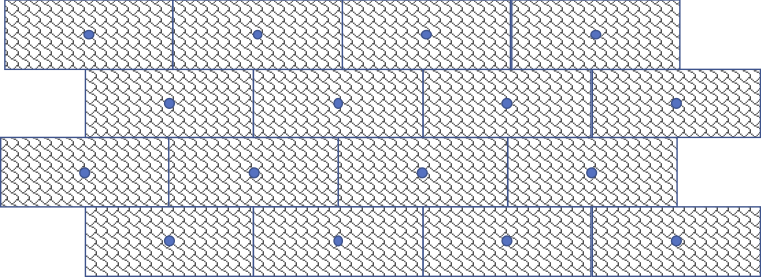
\includegraphics[width=0.6\linewidth]{figures/Bricks.png}
    \caption{A 2-D lattice generated from bricks. As a guide for equivalent points, a dot has been placed at the center of each brick.}
    \label{fig:latt1}
\end{figure}
  The problem with the cell to the left (in red) is that it is oblique – the angles between sides are not right angles – and thus we have lost some essential symmetry information about the rectangular bricks. The problem with the cell at the right (in green) is that while it preserves the rectangular symmetry of the bricks, it is twice as large as a single brick and thus is less than optimal in providing the simplest possible description of the lattice. Note that we cannot use a single brick as a unit cell, because that would violate the principle that a unit cell translation of applied to a point in any direction provides an identical point. Translation vertically by one unit would take a point from the middle of one unit cell to the edge of another. 
\begin{figure}
    \centering
    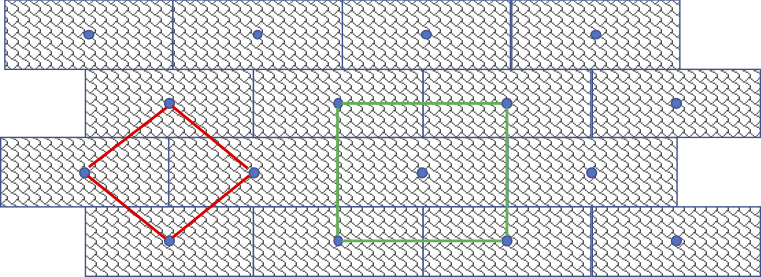
\includegraphics[width=0.6\linewidth]{figures/Bricks2.png}
    \caption{Two different unit cells, that will create the pattern in previous figure. The one in read does not show that the lattice symmetry is rectangular (orthorhombic).}
    \label{fig:latt2}
\end{figure}
 Lattice centering provides a secondary rule for lattice generation which places lattice points not only at the corners of unit cells but also at locations within cells. If we label axes above so that we are looking at the x-y plane and call the corners of the green box as (0,0,0), (1,0,0), (0,1,0) and (1,1,0) then we can also label the central point between them as (½, ½, 0). We already have said that adding any number of unit cell translations brings us to a point that is equivalent to our original point, which we can write algebraically as saying that point (x,y,z) is equivalent to (x+n\textsubscript{x},y+n\textsubscript{y},z+n\textsubscript{z}), where n\textsubscript{x}, n\textsubscript{y}, n\textsubscript{z} and n\textsubscript{c} can each be any integer. To express the idea that the environment of (½, ½, 0) is the same as (0, 0, 0) we can write an additional equivalence, that point (x,y,z) is equivalent to (x+n\textsubscript{x}+½ , y+n\textsubscript{y}+½, z+n\textsubscript{z}), where again n\textsubscript{x}, n\textsubscript{y}, n\textsubscript{z} and n\textsubscript{c} can each be any integer. 

 This brings us to the concept of a \textbf{symmetry operation},\index{symmetry operation} which will be needed when we discuss space groups. We use these only to describe the symmetry within the unit cell, so we do not need to consider the translations above, where we added integers to x, y or z as that relates the contents of one unit cell to a neighbor. However, one requirement of mathematical groups is that they must contain an identity operator, so even if there is pattern of repetition within the cell, the identity symmetry operation x,y,z must be present. However, in the case of the centering operation with our bricks, we can write a symmetry operator ½+x,½+y,z meaning that if we place an atom at coordinates (x,y,z), we automatically generate another a half unit cell away in both x and y. Note that if x>1/2 then x+½ will be in the next unit cell, but we can add or subtract any integer from x to translate back into the current unit cell, so ½+x+n\textsubscript{x},½+y,z is implied by ½+x,½+y,z and thus is equivalent to x-½,½+y,z.

 Lattice centering is most useful for crystal classes where the centered lattice demonstrates some symmetry that the \textbf{primitive lattice}\index{primitive lattice} (as we call a same lattice without centering) does not. If we place a lattice center into the middle of a triclinic cell, with coordinates (½, ½, ½) or equivalently consider this as the symmetry operation ½+x, ½+y, ½+z, it will have a doubled volume in comparison to any of the smallest possible primitive cells, but provides no extra symmetry information. This does not mean that it is illegal to use a centered description with a triclinic unit cell, in fact it may be useful for understanding what is changing when a material transforms from a structure with a centered cell to one that is triclinic, but the standard descriptions will not include any centered triclinic cells. In contrast, if we take an orthorhombic cell with a body center, we can construct several primitive cells, but none will have the three perpendicular axes found in the centered cell. Thus, centering allows us to demonstrate the full symmetry of that orthorhombic lattice. 

 There are two types of centers needed to construct the possible symmetry types for all three-dimensional lattices, known as the Bravais lattices\index{Bravais lattice}. One center type is placed in the side of a unit cell and called a face center. A face center with coordinates (½, ½, 0) is in the face perpendicular to \textit{c} and is called a C-center. Likewise, centers at (½, 0, ½) and (0, ½, ½) are called B-center and A-centers, respectively. As we saw before, a center at the middle of the unit cell is called a body center or is abbreviated as an I-center (short for the German word \textit{Innenzentriert}.). Combinations of centers are possible, but the only combination that cannot be simplified without loss of the underlying symmetry is when A-, B- and C-centers are \textit{all} combined. This combination is referred to as face centering or an F-center. Note that a A-, B-, C- or I-center will double the number of symmetry operations while face centering leads to four symmetry operations x,y,z; ½+x,½+y,z; ½+x,y,½+z; and x,½+y,½+z. Sometimes the expanded volume of a centered lattice is referenced by comparison to the low-symmetry primitive unit cell. Thus, a A-, B-, C- and I-centered lattice is doubly-primitive, meaning the centered cell has double the volume of the primitive cell. An F-centered lattice is quadruply-primitive. It is also possible to consider a lattice center on an edge of a unit cell, such as (½,0,0). Edge centers are used for description of unit cells for magnetic scattering but are not needed for the 14 Bravais lattices. 

 There is one special case of centering specific to related to rhombohedric unit cells. It is possible to transform any lattice constructed from rhombohedric unit cells (a=b=c, α=β=γ) into one that has a=b, γ=120° and α=β=90° unit cells,e.g. the same cell as a hexagonal lattice but this cell has three times the volume of the primitive rhombohedric unit cell and with lattice centers at (2⁄3, 1⁄3, 1⁄3) and (1⁄3, 2⁄3, 2⁄3). We use the symbol R is used for this type of centering. While both types of unit cells are used for this system because the same lattice can be generated either from a primitive rhombohedron or a triply-primitive centered cell in a hexagonal lattice, the hexagonal description tends to be used more commonly because it is usually somewhat more computationally simple.

\begin{table}
\centering
\caption{The 14 Bravais lattices as distributed across the 7 crystal systems, where P indicates a primitive cell, F for centers on all faces, I for a body center, R for rhombohedral centering (see text) and C for a C-center. Note that face centers can be interchanged between A, B and C-centering by relabeling axes.}
\begin{tabular}{| l | p{0.13\textwidth} | p{0.3\textwidth} | p{0.23\textwidth} |}
\hline
Name & Constraints on lengths & Constraints on angles & Bravais lattice centering options \\
\hline
Cubic & \textit{a}=\textit{b}=\textit{c} & α = β = γ = 90° & P, F, I \\
\hline
Tetragonal & \textit{a}=\textit{b} & α = β = γ = 90° & P, I \\
\hline
Orthorhombic & none & α = β = γ = 90° & P, C, F, I \\
\hline
Hexagonal & \textit{a}=\textit{b} & γ = 120°; α = β = 90° & P \\
\hline
Rhombohedral & \textit{a}=\textit{b}=\textit{c} & α = β = γ & R \\
\hline
Monoclinic & none & b unique: α = γ = 90° & P, C \\
\hline
Triclinic & none & none & P \\
\hline

\end{tabular}

\end{table}


\section{Crystallographic Symmetry Elements}

 So far, we have not considered where atoms are located within the unit cell, but it should come as no surprise that symmetry plays a role in that, too. If you have studied point group symmetry and not crystallographic symmetry, you have learned about two types of symmetry axes, proper and improper rotation axes, which are defined slightly differently in crystallographic use. However, point group symmetry does not include two additional types of symmetry that involve translations: screw axes and glide planes. Before reviewing these four types of symmetry elements, let’s dive deeper into the notation used to describe symmetry operations and their algebra. We use the concept of an operator to describe how a duplicate atom is created from the initial position with a triplet of formulae, \textit{f}\textsubscript{x},\textit{f}\textsubscript{y,}\textit{f}\textsubscript{z}, where each of the \textit{f}\textsubscript{i} is an algebraic expression dependent on x, y \& z. 

 As we saw, if we take an atom at position x,y,z and we have a body center in that lattice, this means that for every atom in the unit cell, there is another identical atom displaced from that atom by a half unit cell in each direction. We can write that as an operator as ½+x,½+y,½+z. We understand this operator to mean that we create a new atom from the first with its coordinates shifted by half unit cell translations. If the coordinates of the original atom is x,y,z and the coordinates of the second atom are x’,y’,z’, then x’=½+x, y’=½+y, z’=½+z. Likewise if we consider another symmetry operator, ½+y,-x,z, then that creates a copy of that atom where x’= ½+y and y’=-x but z’=z. 

 Symmetry can also be written as a matrix and vector. In this notation ½+y,-x,z would be written as 
 
$$\begin{matrix}x\prime\\y\prime\\z\prime\end{matrix}=\ \left[\begin{matrix}0&1&0\\-1&0&0\\0&0&1\end{matrix}\right]\left[\begin{matrix}x\\y\\z\end{matrix}\right]+\left[\begin{matrix}{1/2}\\0\\0\end{matrix}\right]$$

Let’s now consider a mirror plane symmetry operation, where we will place that symmetry element in the x,y-plane and at z=½. What does that mirror plane do? Viewed along the \textit{c} direction, perpendicular to the mirror plane, it appears to do nothing, because x and y will be unchanged by the action of the mirror plane. So, we can see the new position has the same values of x and y. Viewed from a direction in the plane of the mirror (for example, viewing along \textit{a} or \textit{b}), it becomes clear that the mirror plane involves a change in the z value to z’. A bit of thought makes clear that whatever the distance from the atom to the mirror plane, that distance must stay the same, but the atom will lie on the opposite side of the mirror plane. So, if our atom is at position z, then the distance to the mirror plane is |½-z| and the direction from the atom to the mirror plane will be along a vector from z to ½. For simplicity in visualization, we will assume 0 < z < ½, but what here is true for all values of z, assuming that a periodic lattice is present, so that adding or subtracting any multiple of one from z yields an indistinguishable value. The position on the other side of the mirror plane with the same distance to the mirror plane will be z’ = 1-z. We can see that |½-(1-z)| which is equal to |z-½|. Thus, we can say that our mirror plane in the x,y-plane and at z=½ is equivalent to a x,y,1-z operation. Since we can add or subtract any multiple of one to x, y and/or z, a simpler form for this operator is x,y,-z. Crystallographers have an even more compact notation for this, written as $x,y,\bar{z}$, where the last term is called “z bar” and means -z. Modern software does not make $\bar{z}$ easy to type, so I will use this notation sparingly.

There are two things we can learn from this x,y,-z operator. One is the idea of \textbf{special positions}, which is demonstrated by what happens if we have an atom that is placed on the mirror plane, meaning that that z=½ (note that x \& y are arbitrary). We can designate this in a more compact notation, as position (x,y,½). Applying this x,y,-z operator to position (x,y,½) generates position (x,y,-½). Since adding any positive or negative multiple of 1 to any coordinate generates an equivalent position in the lattice, the positions (x,y,½) and (x,y,-½) are indistinguishable and thus while in general an atom placed at (x,y,z) generates a second atom at (x,y,-z), the position (x,y,½) is special; we do not actually generate a new position for any atom with z=½. Thus, we say that due to the presence of this mirror plane, atoms at (x,y,½) are at special positions, because if there are \textit{n} atoms on one side of the mirror plane, then the mirror plane will generate a second set of \textit{n} atoms on the other side of the mirror plane and thus the unit cell must contain 2\textit{n} atoms, but not so for the atoms on the special position (x,y,½) because there will no duplicates for the atoms that lie on the mirror plane. The unit cell contents will thus be A\textsubscript{2n}B\textsubscript{n} where the B atoms have z=½ [or as we will see where z=0, as (x,y,0) is also a special position.] 

The second concept is that the presence of symmetry operators in combination with each other and/or the lattice can create additional symmetry operations. To understand how one symmetry operation can modify another operation, note that -x,-y,-z is equivalent to replacing the expression for x’,y’ and z’ with those values multiplied by -1. If we combine the -x,-y,-z and x,y,z symmetry operations this yields the original symmetry operation -x,-y,-z. If we apply -x,-y,-z to symmetry operation -x,y,½+z we get x,-y,½+z [note that -1*(½-y) is y-½ but in an lattice adding 1 but the completely equivalent position, ½+z, is preferred by convention.] Let us consider what happens with a mirror plane in the x,y-plane placed at z=0. This will “reflect” any atom at position z to z’=-z. The operator form of this is also x,y,-z, which is also identical to the operator created by the mirror plane at z=½. Thus, the presence of a lattice and a mirror plane at z=½ (and at –½, 1+½,…) requires the presence of an additional set of mirror planes at z=…-2,-1,0,1,2,… Likewise, a mirror plane at z=0 cannot exist without a mirror plane at z=½.

Now let us review the four types of symmetry elements.

\subsection{Proper rotations} Proper rotations are defined relative to a line and by the fraction of a circle that is rotated. Thus, to fully describe a proper rotation, we need to specify a direction relative to the \textit{a}-, \textit{b}-, and \textit{c}-axes and a point that the axis travels through and finally the fraction of a circle for the rotation (example: a 3-fold axis along \textit{a} that passes through y=z=¼.) The only rotations that are possible in crystals are 1-fold, 2-fold, 3-fold, 4-fold and 6-fold and the Bravais lattice dictates which of these are allowed. Thus, an N-fold rotation produces rotations of 360°/N (2p/N radians). Not all proper rotation axes can be found in any given Laue class. For example, a triclinic cell is not compatible with any rotation axis other than 1-fold. A 4-fold rotation axis interchanges axes and thus requires a minimum of two equivalent length axes (cubic and tetragonal cells), while a 3-fold axis requires a rhombohedric or hexagonal cell. A 6-fold rotation axis can only exist in a hexagonal cell. The symbol used for a N-fold proper rotation axis is simply the number 2,3,4,6 (no symbol is needed for the 1-fold)

Table \ref{tab:proper} shows the coordinates for atom positions generated by a proper rotation axis along the c-axis passing through x=y=0. Note that a 1-fold rotation axis is simply the identity operation. It generates only the original position of an atom. 
 
\begin{table}
\centering
\caption{Positions generated by a \textit{n}-fold proper rotation axis parallel to \textit{c} and passing through x=y=0}
\label{tab:proper}
\begin{tabular}{| p{0.1\textwidth} | p{0.075\textwidth} | l | l | l | l | l | l |}
\hline
Axis type & symbol & \multicolumn{6}{l|}{Generated atom positions} \\
\hline
1-fold &   & (x,y,z)  &   &   &   &   &   \\
\hline
2-fold & \textbf{2} & (x,y,z) & (-x,-y,z) &   &   &   &   \\
\hline
3-fold & \textbf{3} & (x,y,z) & (-y,x-y,z) & (y-x,-x,z) &   &   &   \\
\hline
4-fold & \textbf{4} & (x,y,z) & (-y,x,z) & (-x,-y,z) & (y,-x,z) &   &   \\
\hline
6-fold & \textbf{6} & (x,y,z) & (x-y,x,z) & (y,y-x,z) & (-x,-y,z) & (y-x,-x,z) & (-y,x-y,z) \\
\hline

\end{tabular}

\end{table}

\subsection{Improper rotations} Proper rotations are defined relative to a line for the rotation axis, but also a point along that axis. Thus, to fully define an improper rotation axis one needs the rotation order, a point and an axis of rotation. The way that improper rotations are applied is to first perform an inversion operation through the defined point and then apply the rotation, as was done with proper rotations. (Note that improper rotations, as used in molecular point group symmetry, are defined slightly differently and the Schoenflies labels work slightly differently; the crystallographic conventions are, of course, better.) Again, the improper rotation axes are named by the fraction of a circle that is rotated and again, only the only improper rotations that are possible are 1-fold, 2-fold, 3-fold, 4-fold and 6-fold, where only some of these are consistent with each Bravais lattice. Below is a table showing the coordinates for atom positions generated by an improper rotation axis along the c-axis and point x=y=z=0. The symbol used for a N-fold improper rotation axis is simply the number with a horizontal line above, as seen in the table. Note that the $\bar{1}$ operation is simply an inversion center, also sometimes called a center of symmetry. This does not have an axial direction, but does have an origin location. The $\bar{2}$ operation is simply a mirror plane. This is defined relative to a plane, but has no origin. Table \ref{tab:improper} shows the coordinates for atom positions generated by an improper rotation axis along the c-axis passing through x=y=0.

\begin{table}
\centering
\caption{Positions generated by a \textit{n}-fold improper rotation axis parallel to \textit{c} and passing through x=y=0}
\label{tab:improper}

\begin{tabular}{|  p{0.08\textwidth} | p{0.08\textwidth} | l | l | l | l | l | l |}
\hline
Axis type & symbol & \multicolumn{6}{l|}{Generated atom positions} \\
\hline
1-fold & \vspace{0.01mm}$\bar{1}$ & (-x,-y,-z)  &   &   &   &   &   \\
\hline
2-fold & \vspace{0.01mm}$\bar{2}$ & (x,y,z) & (x,y,-z) &   &   &   &   \\
\hline
3-fold & \vspace{0.01mm}$\bar{3}$ & (x,y,z) & (x-y,x,-z) & (-y,x-y,z) & (-x,-y,-z) & (y,y-x,-z) & (-y,x-y,z) \\
\hline
4-fold & \vspace{0.01mm}$\bar{4}$ & (x,y,z) & (-y,x,-z) & (-x,-y,z) & (y,-x,-z) &   &   \\
\hline
6-fold & \vspace{0.01mm}$\bar{6}$ & (x,y,z) & (y-x,-x,z) & (-y,x-y,z) & (x,y,-z) & (y-x,-x,-z) & (-y,x-y,-z) \\
\hline

\end{tabular}

\end{table}

\subsection{Screw axes} 
So far, we have seen point symmetry in the form of proper and improper rotations and the only translational symmetry we have seen is in the form of unit cell translations. There is also a symmetry operation that combines both rotational symmetry and translation. These are called screw axes and these describe helictical symmetry in a material. A screw axis has a defined translation direction and a location in the plane perpendicular to that direction. A screw axis is labeled N\textsubscript{m} where the first number, N, (2, 3, 4 and 6) describes the amount of the rotation, where the rotation is 360°/N (2p/N radians) so a 2\textsubscript{1} screw axis will cause a 180° rotation (generating 2 positions), while a 6\textsubscript{m }screw axis will have 60° rotations. The second number, m combined with N (the first), dictates the translation amount as m/N, so the translation is a half unit cell for a 2\textsubscript{1 }screw axis and one-sixth of a unit cell for a 6\textsubscript{1 }screw axis. Thus, a 2\textsubscript{1}screw axis will duplicate an atom (two atoms/cell) and a 6\textsubscript{1 }screw axis will create five copies (six atoms/cell). The crystallographically defined screw axes are 2\textsubscript{1}, 3\textsubscript{1}, 3\textsubscript{2}, 4\textsubscript{1}, 4\textsubscript{2}, 4\textsubscript{3}, 6\textsubscript{1}, 6\textsubscript{2}, 6\textsubscript{3}, 6\textsubscript{4} and 6\textsubscript{5}. Screw axes can occur along the \textit{a}, \textit{b} or \textit{c} directions or in three-fold symmetry materials (cubic and rhombohedric cells, along the body-diagonal, the 111 direction.) Thus, a full description of a screw axis will specify the type, the direction and a location of the axis, usually by giving a point that the axis travels through. 

 For an example, let us consider a 4\textsubscript{1} screw axis along the \textit{c} axis through the point x=y=0. The rotation portion of the axis will transform the in-plane coordinates of the atom from (x,y) to (-y,x) and then to (-x,-y) and finally to (y,-x) while simultaneously adding a ¼ unit cell translation. Thus, if we have an atom at coordinates (x,y,z) the generated positions are (-y,x,z+¼), (-x,-y,z+½) and (y,-x,z+¾).

 Note that since unit cell translations are applied in combination with screw axes, the translation of 5/6\textsuperscript{th} of a unit cell is the same as a translation of 1/6\textsuperscript{th} of a unit cell in the negative direction, thus a 6\textsubscript{1} and 6\textsubscript{5 }screw axes are an enantiomeric pair, that differ only in the rotation direction, where the 6\textsubscript{1} screw axis produces a right-handed helix and 6\textsubscript{5 }screw axis produces a left-handed helix. (The same is true for 3\textsubscript{1}/3\textsubscript{2}, 4\textsubscript{1}/4\textsubscript{3,} and 6\textsubscript{2}/6\textsubscript{4}.) Thus, the 4\textsubscript{3 }screw axis describes a helix with the opposite rotation direction of the 4\textsubscript{1} axis shown before, with generated coordinates (x,y,z), (y,-x,z+¼), (-x,-y,z+½) and (-y,x,z+¾). Note that while a 4\textsubscript{1} and a 4\textsubscript{3} axes will be found in different space groups, with powder diffraction all the reflections that could be sensitive to this rotation direction (due to anomalous dispersion) are superimposed, so it is impossible for a powder diffraction experiment to differentiate the enantiomeric handedness for a material. Without some other type of data, the distinction between each pair of related symmetry elements can be ignored. Space group \textit{P}6\textsubscript{1} and \textit{P}6\textsubscript{5} are considered different space groups as they can accommodate objects of with different handedness, but to powder diffraction they are the same. 

\subsection{Glide planes} The last type of symmetry element found in crystals combines translation and reflection and is called a glide plane. A glide plane causes an atom to be translated by a half-unit cell in one direction and then reflected through a plane. We name the glide plane for the translation direction (as an a-glide, b-glide or c-glide), but the full description for a glide plane will also name the reflection plane by specifying the perpendicular axis (which obviously must be a different axis than the translation direction.) If we take for example a c-glide perpendicular to \textit{a}, which I placed at x=0, we can see that the reflection operation will take (x,y) and transform that to (-x,y) the translation of a half-unit cell adds to z. Thus, coordinates (x,y,z) are transformed to (-x,y,z+1/2).

There are few special types of glide planes. An \textit{n}-glide, which is sometimes called a diagonal glide, is similar to a a-glide, b-glide or c-glide except that the translation is applied along two axes and the glide is named for the axis normal to the reflection plane. One must specify the coordinate along this axis to know where te . As an example, in space group \textit{Pn} there is a n-glide perpendicular to \textit{b} at y=0. This will cause an atom to be reflected from y to -y followed by a translation along both a and c, thus the operator for this will be ½+x, -y, ½+z. 

 A \textit{d}-glide, sometimes called a diamond glide, involves a reflection followed by a translation along either a face-diagonal direction (translating along a+b, or a+c, or b+c, or any positive or negative permutation, such as a-b, -a-b or -a+b) or a body-diagonal direction (which can be any of the 6 directions permuting +a, -a, +b, -b and +c,-c). However, the translations for a d-glide is a quarter of a unit cell unlike all other glide plane types. Note that d-glides are only found in body-centered (I) and face-centered (F) lattices. A specify a d-glide, one needs to indicate the direction of the translation as well as the location and orientation of the reflection plane. As an example, a d-glide along the 110 diagonal and perpendicular to \textit{c} at z=0 will have operator ¼+x,¼+y,-z. 

\section{Space groups}

The mathematical concept of a group is a bit different from the sort of practical math that is most commonly taught, such as algebra, trigonometry and calculus, but one of the great discoveries (of the 18\textsuperscript{th} century) when it comes to describing the possible types of symmetry that can be found in isolated objects (point groups) or objects in a lattice (\textbf{space groups}). Returning to the operators For our purposes, we can consider these operations as the symmetry actions that will determine the positions of atoms in our unit cell. 

Groups are built from operators, which for our purposes we will consider as giving us the coordinates for duplicate copies of atoms at other locations, as we saw before. To give this important mathematical concept a very brief overview, the key mathematical requirements of a group are that every group must have an identity operation and that group must be complete, meaning that any operator in the group if performed on another operator in a group will generate an operator that is also contained in the group. This means that all permutations of each operator combined generates an operator in the group. This also requires that there must be an inverse operator for every operator in the group.

 We will write the \textbf{identity operation }as x,y,z, meaning that an atom with coordinates (x,y,z) is placed at those coordinates. The simplest group has only this operation and we can see that this group is complete, meaning that any repeated set of operators from the group, in any order, will only create another operator in the group. Thus, a single operator, x,y,z, creates our simplest group, since x,y,z operated on x,y,z gives us the original operator back. This, combined with a translation operators from an infinite lattice, is labeled by crystallographers as \textit{P }1 using what is known as the Hermann-Mauguin space group notation. 

 If we consider the mirror plane operator we saw before, x,y,-z, and combine that with x,y,z, we create a second group with just two elements, since x,y,-z operated on itself gives x,y,z and x,y,-z operated on x,y,z gives back x,y,-z. Combined with a lattice, these two operators will generate a space group \textit{P m} using short-form Hermann-Mauguin notation (or \textit{P }1 1 \textit{m} in long-form Hermann-Mauguin notation, where the 1 indicates there is no symmetry along the \textit{a}or \textit{b} axes.) Some head-scratching about mirror planes will show that a lattice must have an axis that is at right angle to the mirror plane (if not lattice points will not be reproduced at the correct positions), so \textit{P m} is only consistent with a monoclinic unit cell. When I say only consistent with monoclinic, this does not preclude a unit cell that appears to be of higher symmetry, for example it could have all three cell axes appear as 90° within arbitrarily small experimental errors, but only one of these angles is constrained by symmetry to be 90° and thus the cell would not be considered to be orthorhombic unless additional symmetry is present that requires all angles to be 90°.

 We can also take the \textit{P m} space group and add an additional centering operation to create a new space group. Let’s add a B-center which means operator ½+x,y,½+z. When this is operated on x,y,-z we create fourth additional operator, ½+x,y,½-z. Using these four operators on each other, we generate no others. Thus, the space group \textit{B }1 1 \textit{m} has four operators: x,y,z; x,y,-z; ½+x,y,½+z; and ½+x,y,½-z. Note that we used only two symmetry operations (the mirror plane and centering) to generate these four operators. We call those two operators the \textbf{generators} because those two operators can be used generate the entire group and those generators are thus included in the Hermann-Mauguin name. It is also worth noting that Volume A of the \textit{International Tables for Crystallography} does not include \textit{B} 1 1 \textit{m} as one of the 230 space groups, but a closer look at the volume one can find \textit{B }1 1 \textit{m} as one of the non-standard settings for space group \textit{A }1 \textit{m }1. 
 The 230 three dimensional unique space groups tabulated in the \textit{International Tables for Crystallography, Volume A} only reflects only the standard settings for space groups. 
 Just as the \textit{International Tables }lists \textit{B}\ 1\ 1\ \textit{m} as one of the non-standard settings for space group \textit{A}\ 1 \textit{m}\ 1, one could also consider F centering or I centering with a mirror plane and generate other versions of space groups. 
 There are a large number of non-standard space groups. 
 These can always be reduced or transformed to one of the 230 standard space groups, but there can be good reasons why use of a non-standard space group can be very convenient, most commonly because it allows direct comparison of coordinates between related structures. 
 As we will see, GSAS-II does allow you to use these non-standard settings, and they can be quite useful. 

 We saw before that the combination of operations -x,-y,-z and -x,y,½+z generates x,-y,½+z. Thus, we know that -x,-y,-z and -x,y,½+z alone cannot form a group, but you can convince yourself that the four operators, x,y,z, -x,-y,-z, -x,y,½+z and x,-y,½+z do constitute a group. 

 When considering classes of space groups, one must consider that a hexagonal cell can host a structure with a 6-fold (or $\bar{6}$) rotation axis or a 3-fold (or $\bar{3}$). The later are considered trigonal space groups and the former hexagonal. Since rhombohedral symmetry can also be expressed in a hexagonal cell, they are labeled as a special centered case within the trigonal space groups and are given an R prefix. 

\section{Systematic Extinctions}

An important consideration of symmetry is that translational symmetry, where atoms are offset from their original positions by a fixed amount, will cause classes of reflections to have zero intensity, known as systematic extinctions or systematic absences. Only translational symmetry operations (cell centering, screw axes and glide planes) can cause systematic extinctions, while the presence of proper and improper rotation operations do not cause systematic extinctions except in combination with translational symmetry. 

To understand how systematic extinctions arise, let us consider a unit cell with a C-center. To simplify we will assume that the unit cell has only two atoms, if the first is at x,y,z then the second will be at x+1/2, y+1/2, z. If take the structure factor equation, 

$$F_{hkl}=\sum_j^N f_j \exp⁡[-2πi(hx_j + ky_j + lz_j)]$$

and expand this over our two atoms, we get 

$$F_{hkl} = f_j \exp⁡[-2πi(hx_j + ky_j + lz_j)] f_j + \exp⁡[-2πi(hx_j + ky_j + lz_j) + \frac{h+k}{2}] $$

which can be rewritten as 

$$ F_{hkl} = f_j \exp⁡[-2πi(hx_j + ky_j + lz_j)] f_j + \exp⁡[-πi(h + k)] \exp⁡[-2πi(hx_j + ky_j + lz_j) ] $$

Note that when h + k is even, then $\exp⁡[-πi(h + k)] = 1$ but when h + k is odd then $\exp⁡[-πi(h + k)] = -1$ so the sum of the two exponentials is zero. Thus, for C-centering with any number of atoms in the unit cell,  $F_{hkl}=2\sum_j^{N/2} f_j \exp⁡[-2πi(hx_j + ky_j + lz_j)]$ for h+k even, and $F_{hkl}=0$ for h + k odd. 

We can also rationalize this by thinking that if viewed along a reciprocal space direction, symmetry causes the unit cell repeat distance to decrease by a half, then half of the reflections in that projection must disappear. For a 2\textsubscript{1} screw axis along \textit{a}, the viewed along the \textit{a*}-axis, the cell will appear to be half the original size. Thus, \textit{h}00 reflections will be absent when \textit{h} is odd. This only occurs in projection along \textit{a*}. From any other direction this superposition is broken. Likewise, for a \textit{c}-glide plane perpendicular to the \textit{b}-axis, this appears to halve the c-axis length except when not perpendicular to \textit{b}*, so \textit{h}0\textit{l} reflections must have zero intensity when \textit{l} is odd.

 \section{Site symmetry and the asymmetric unit}\label{ref:asymmetricunit}
As noted before, some space groups have locations where if an atom is placed, some symmetry operations will generate the same position again rather than a different location. These are called special positions, which may be a point, line or even plane. For every space group, the \textit{International Tables} has a tabulation of special positions known as the Wyckoff sites. These consist of a number followed by a letter. The number indicates the number of these type of positions that occur in the cell, which is known as the multiplicity. The letter is assigned sequentially. The first item, will have the largest multiplicity, and the last assigned letter will be the the lowest symmetry locations in the cell and with it will be listed the equivalent locations. The subsequent Wyckoff sites will have higher symmetry and lower multiplicity and the locations where that occurs. If a line, it will be expressed as a formula such as (x,0,0) or (x,x,0) and if a plane (x,y,0). 
As an example, the space group $P 2_1/c$ has the following Wyckoff sites listed:

\begin{itemize}
    \item 4e:  $(x, y, z)$; $(\bar{x}, y+\frac{1}{2}, \bar{z}+\frac{1}{2})$; $(\bar{x}, \bar{y}, \bar{z})$; $(x, \bar{y}+\frac{1}{2}, z+\frac{1}{2})$
    \item 2d: $(\frac{1}{2}, 0, \frac{1}{2})$; $(\frac{1}{2}, \frac{1}{2}, 0)$
    \item 2c: $(0, 0, \frac{1}{2})$; $(0, \frac{1}{2}, 0)$
    \item 2b: $(\frac{1}{2}, 0, 0)$; $(\frac{1}{2}, \frac{1}{2}, \frac{1}{2})$
    \item 2a: $(0, 0, 0)$; $(0, \frac{1}{2}, \frac{1}{2})$ 
\end{itemize}
The 4e Wyckoff site is the general position and the other four Wyckoff sites are pairs of discrete points in the unit cell. Alas, the listing order of Wyckoff sites, other than in decreasing multiplicity, is not in any derivable sequence and thus is only a reference to the \textit{International Tables} tabulations. I tend to avoid use of Wyckoff labels as I consider the letter assignment to be arbitrary. 

Related to site multiplicities is the concept of the asymmetric unit. This can be expressed in two different ways. The \textit{International Tables} lists an asymmetric unit for each space group as a unique volume within the unit cell and if that unique volume is duplicated using the symmetry operators, the entire contents of the unit cell can be constructed. The other way that the asymmetric unit is described is in terms of the unique atoms that can be used to build up the unit cell contents. Note that each atom in the asymmetric unit will then have a multiplicity. The previous expression for the structure factor can then have the number of terms reduced

$$F_{hkl}=\sum_j^{N^\prime} f_j m_j\exp⁡[-2πi(hx_j + ky_j + lz_j)] \exp⁡[-2πi(\vec{Q}\cdot\vec{U_j})]$$

where the summation over $N^\prime$ reduced to a summation over the number of atoms in the asymmetric unit rather than the entire unit cell contents and an extra term, $m_j$, is included for the multiplicity of each atom site. 

\section{Space groups in GSAS-II}

In GSAS-II, to simplify the listings of the symmetry operations, they are shown in a manner that minimizes the number of operators that must be provided. This is done by providing only the unique operators, if there is a center of symmetry and lists the centering operations. The full set of operations will be created by applying the center of symmetry and centering operations to the unique operators. An example will show how this works. For the space group, \textit{F }2/\textit{c} (which is a non-standard setting of the monoclinic space group \textit{P }2/\textit{c}) there are 16 symmetry operations, 
\begin{center}
x,y,z \\
-x,y, ½-z \\
-x,-y,-z\\
x,-y,z+½\\
x,y+½,z+½\\
-x,y+½,-z\\
-x,½-y,½-z\\
x,½-y,z\\
x+½,y,z+½\\
½-x,y,-z\\
½-x,-y,½-z\\
x+½,-y,z\\
x+½,y+½,z\\
½-x,y+½,½-z\\
½-x,½-y,-z\\
x+½,½-y,z+½
\end{center}

GSAS-II displays the window in Fig. \ref{fig:F2_c}
for this space group.

\begin{figure}
    \centering
    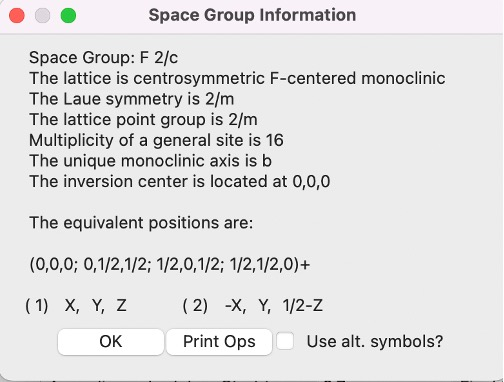
\includegraphics[width=0.5\linewidth]{figures/F2_c.jpg}
    \caption{Information displayed by GSAS-II for the non-standard space group $F 2/c$}
    \label{fig:F2_c}
\end{figure}
Note that at the bottom of this window, two unique symmetry operations are given: x,y,z and -x,y,½-z, but as noted the multiplicity of a general site is 16, meaning there must be a total of 16 symmetry operations. The two initially supplied symmetry operations are doubled because this space group is noted as centrosymmetric. Thus, the center of symmetry operation, -x,-y,-z, is applied to each of the two initial symmetry operations, generating two additional operations, -x,-y,-z and x,-y, ½+z. These four symmetry operations are also operated upon by the four centering operations, listed as (0,0,0)+, (0,½,½)+, (½,0,½)+, (½,½,0)+. The first centering operation gives us back the four operators already listed, but adding (0,½,½) to each of these the four operators we already have provides us with four new operations: x,½+y,½+z, -x,½+y,-z, -x,½-y,½-z and x,½-y,z. Likewise, applying the (½,0,½)+, (½,½,0)+ operations will generate the other 8 symmetry operations. Thus, we generate all 16 of the operators listed above. Pressing the “Print Ops” button causes these 16 operations to be displayed in the GSAS-II console window. 

The use of these grouped operators allows the most complex space groups (which have 192 operators) to be shown in GSAS-II with only 24 basic operators, where these 24 operators will be doubled to 48 by a center of symmetry, and then each of the three additional centering operators will provide another 48 operators giving us a total of 192 (=24*2*4).

 Space groups are input to GSAS-II with a space between each set of symmetry operations, so the space group \textit{P}6\textsubscript{3}/\textit{mmc} will be specified as \texttt{P 63/m m c}, though for standard settings, space group symbols will be recognized even if the spaces have not been specified correctly. 

One place where GSAS-II is quite restrictive is with centrosymmetric space groups where the highest symmetry location in the cell is not a center of symmetry. Such space groups are documented in the \textit{International Tables} with two choices for origin. In the first origin setting ("Origin 1")\index{Origin 1}, the highest symmetry position is selected as (0,0,0), while Origin 2\index{Origin 2} places a center of symmetry at (0,0,0). Origin 2 is computationally much simpler (since reflection phases are real). GSAS-II only accepts structures in Origin 2 settings in those space groups where there is a choice. When a structure is imported into GSAS-II where this choice exists, if symmetry operators are in the file (currently only in some CIFs), and an Origin 1 setting is detected, GSAS-II will perform the necessary translation to place the structure into Origin 2. Without symmetry operators, the origin can not be determined automatically, but atom multiplicities are computed using both origin settings and usually it is clear which origin setting will provide the correct stoichiometry. As a last resort, plotting of the structure will almost always make it very clear if a reasonable bonding geometry is being generated. If the origin setting is wrong, the generated diffraction pattern will also be wrong. 

Finally, in rhombohedral space groups, the cell is assumed to be hexagonal. To specify that the primitive rhombohedric cell should be used, add a final letter “r” to the space group name. Thus, “R 3” will provide symmetry for a hexagonal cell, but “R 3 r” will provide the symmetry for a rhombohedric cell. Usually, refinements are more stable with the hexagonal cell. 